
%---------------------------------------%
% Packages arranged by : Tsz Timmy Chan %
%                 Date : May 26th, 2019 % 
%---------------------------------------%

\documentclass{TC}
\usepackage{TCcommon}

\title{TITLE HERE}	% Work Title Here.
\author{Tsz Timmy Chan}	% YOUR NAME HERE 

\usepackage[notes]{TCheader}
\usepackage{TCexamtitle}

\usepackage{setspace}
\linespread{1.5}

%\renewcommand{\benediction}{" " - }
%\renewcommand{\quoteoftheday}{" " \\ - }

\begin{document}
Then on the next chapter, it's a tiny bit more readable but still pretty dense, almost math textbook dense \parencite{green_epistemology_2006}.
	\begin{itemize}
	\item Pages on critiques of positivist focus, boiled down to...
		\begin{enumerate}
		\item Strong theory-dependence; i.e., observations, choices of procedures, and inferences made from data are dependent on the beliefs one holds about the world. Observations are not independent of the intellectual apparatus brought to bear on the objects of concern; finding observations that are truly indubitable was formidable, given variation in observer knowledge and perspective. 
		\item Data seem to underdetermine theory choice- there are instances in the history of science to suggest that multiple theories are equally supported by empirical evidence in a given instance.
		\item Any hypothesis is tested empirically, a number of auxiliary hypotheses are assumed at least provisionally true, and so that when a main hypothesis is tested and seemingly refuted, it may be due to an auxiliary hypothesis was mistakenly taken to be true when it was in fact false.
		\item Continual discovery of the social basis of disciplinary knowledge is in contradiction to the formalism of logical positivist epistemologies
		\item Plurality of knowledge systems is derived thru the work of particular epistemic communities.
		\end{enumerate}	
	\item $\exists$ multiple challenges to educational research:
		\begin{enumerate}
		\item Frustration with the degree and usefulness of knowledge relevant to education currently available
		\item Plurality has its advantages and should be encouraged, with a distinction between claims to validity (moral reasoning) and claims to truth (scientific reasoning).
		\end{enumerate}	
	\item One may address the above critiques and challenges through critical discourse, within group, regarding public reason and hermaneutical conversations across groups.
		\begin{enumerate}
		\item Within group --- Developmental and definitional work regarding the creation/specification/extension of research $\rightarrow$ theories, assumptions, ontological commitments. (include socialization of new members)
		\item With public reason --- Development of epistemological commitments to asses value of educational research across traditions $\rightarrow$ internal consistency, empricial adequacy, usefulness for practitioners
		\item Hermaneutics --- 
		\end{enumerate}
	\end{itemize}
	\begin{itemize}[(??)]
	\item Is this a version of pragmatism spoken of in Chapter 1?
	\end{itemize}

Smith Chapter on mixed methodologies \parencite{green_multiple_2006}: 
\begin{itemize}
\item Complex scenarios require mixed methodologies
\item $\exists$ different types and ways to use mixed methodologies
	\begin{enumerate}
	\item sequential design
	\item concurrent design
	\item confirmational
	\end{enumerate}
	
\item \gls{IES} goal structure
	\begin{enumerate}[\text{Goal} 1]
	\item Exploratory
	\item Development, usually uses \gls{dbr}
	\item Efficacy, usually uses \gls{rct} to demonstrate that under optimal conditions that $\exists$ effect
	\item Effectiveness: It worked, but can it be scaled? This is super expensive, typically over 10 million dollars, and most intervention inventions may end here.
	\end{enumerate}
\end{itemize}
Greeno Chapter in the same book \parencite{green_theoretical_2006}:

\begin{figure}[h]
\centering
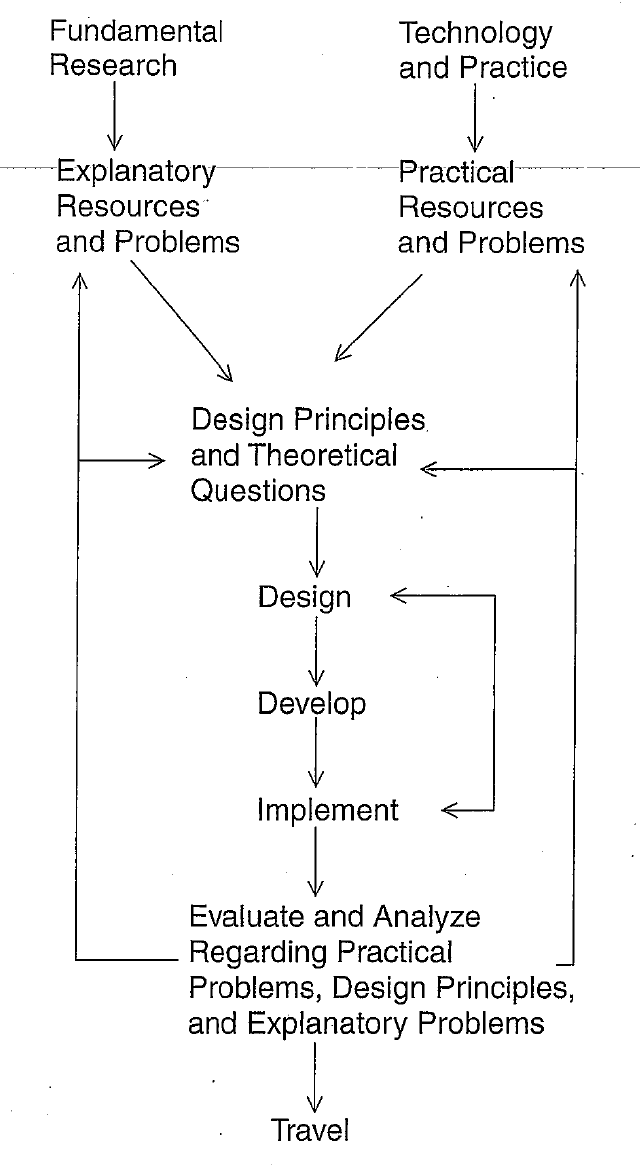
\includegraphics[width=.4\textwidth]{greeno_model_problem_solving_RandD.png}
\caption{Model of Problem Solving R \& D \parencite{green_theoretical_2006}}
\label{fig:Model_of Problem_Solving_R_and_D}
\end{figure}

\begin{itemize}
\item many discussions on the different types of methodologies, with some examples from the progress in math education.
\item Greeno defined design-based research as:

\begin{definition}[design-based research]
A view on research that understands fundamental research as a resource for design and development, includes attention to a body of design principles that can be developed in a field of engineering. See  \autoref{fig:Model_of Problem_Solving_R_and_D} for the pathways involved.
\end{definition}
\end{itemize}






\end{document}
